\documentclass{ltjbook}
\usepackage{docmute} 
\usepackage{../../myStyle} 
\begin{document}

\chapter{RによるWithinデザインの分散分析}
\label{withinDesign_onR}
前回は群内要因(Within Design)の理論について学びました。今回はRを使って実際に群内計画の分散分析を行う方法について学びます。具体的には，\texttt{anovakun}関数を用いて，一要因および多要因の群内計画の分散分析を実行し，その結果を解釈する方法について解説します。また，分析結果の可視化方法についても学びます。

\section{Rとanovakunの準備}
まずはRStudioを起動し，この授業のプロジェクトフォルダを開いてください。
新しいスクリプトファイルを準備して，anovakun関数を読み込みましょう。読み込み方は第\ref{ch20_BetweenDesign_onR}章で説明したとおりですから，忘れた人は確認してください。

\begin{enumerate}
    \item RStudioを起動する。
    \item この授業のプロジェクトを開く。
    \item 新しいスクリプトファイルを開く。一行目に\verb|rm(list=ls())|と書くと尚良い。
    \item anovakun関数を読み込むコードを書く。コードは\ref{code:22_01}の通り。
    \item environmentタブに\texttt{anovakun}関数が読み込まれたことを確認する。
\end{enumerate}

\begin{lstlisting}[language=c++,label={code:22_01},caption={ソースを読み込む}]
# プロジェクトフォルダにソースコードをダウンロードしていればこちら
source("anovakun_489.txt")
# インターネットから直接読み込む場合はこちら
source("https://bit.ly/3WL8VYR")
\end{lstlisting}

\section{一要因Within計画の実際}
さて，準備ができたところで実際にWithin計画の例をやってみましょう。仮想データは前回用いた，次のような表\ref{tbl::22_01}を使います(表\ref{tbl::22_01}と同じものを再掲しています。)。
\begin{table}[ht]
	\centering
	\caption{Within Data Example}
	\begin{tabular}{lrrr}
		\hline
		ID & Time1 & Time2 & Time3 \\
		\hline
		1  & 10    & 5     & 9     \\
		2  & 9     & 4     & 5     \\
		3  & 4     & 2     & 3     \\
		4  & 7     & 3     & 5     \\
		\hline
	\end{tabular}
	\label{tbl::22_01}
\end{table}

これをデータフレーム型にします(\texttt{code:\ref{code:22_02}})。
\begin{lstlisting}[language=c++,label={code:22_02},caption={データフレームにする}]
Example3 <- data.frame(ID=1:4,
Time1 = c(10,9,4,7),
Time2 = c(5,4,2,3),
Time3 = c(9,5,3,5))
\end{lstlisting}

線形モデルとして表現するには，少し複雑な操作が必要ですので，今回は分散分析的アプローチのみ紹介したいと思います。

群内モデルの\texttt{anovakun}での入力は次のようになります(\texttt{code:\ref{code:22_03}})。
\begin{lstlisting}[language=c++,label={code:22_14},caption={anovakunで実行}]
anovakun(Example3[, 2:4], "sA", 3, eps = T)
\end{lstlisting}
データセットや変数の指定，効果量オプションの指定はとくに追記することはありません。デザインの指定が\texttt{"sA"}と\texttt{s}の右側に来ているところがポイントです。これを実行すると，ずらりと結果が示されます。以下，順に結果の読み方を解説します。

\subsection{球状性の検定}
結果の最初に，記述統計と球状性の検定の結果が示されます。出力\ref{RS:out22_01}の箇所を見てください。

\begin{Rscreen}{sAタイプのanovakun出力1;記述統計と球状性の検定}{out22_01}
	\begin{verbatim}
 
<< DESCRIPTIVE STATISTICS >>

--------------------------
  A   n    Mean    S.D. 
--------------------------
 a1   4  7.5000  2.6458 
 a2   4  3.5000  1.2910 
 a3   4  5.5000  2.5166 
--------------------------


<< SPHERICITY INDICES >>

== Mendoza's Multisample Sphericity Test and Epsilons ==

-------------------------------------------------------------------------
 Effect  Lambda  approx.Chi  df      p         LB     GG     HF     CM 
-------------------------------------------------------------------------
      A  1.0000     -0.0000   2 1.0000 ns  0.5000 1.0000 3.0000 0.5000 
-------------------------------------------------------------------------
                              LB = lower.bound, GG = Greenhouse-Geisser
                             HF = Huynh-Feldt-Lecoutre, CM = Chi-Muller
\end{verbatim}
\end{Rscreen}

まず\verb|<< DESCRIPTIVE STATISTICS >>|の部分があります。これは群ごとの平均と標準偏差なので，問題ないでしょう。

次に\verb|<< SPHERICITY INDICES >>|とありますね。これは\keyterm{球状性の検定}{きゅうじょうせいのけんてい}{sphericity test}と訳されます。急によくわからない言葉が出てきて驚かれたかもしれませんが，これが群内要因の分散分析における重要なポイントです。ちょっと長くなりますが，丁寧に説明していきます。
\subsubsection{等分散性の仮定とその拡張}
まず，$t$検定の時にWelchの補正をしたのを思い出してください。$t$検定はその仮定として，2つの群がどちらも正規分布に従い，かつ2つの群の母分散が等しいと考えます。2つの群を$X_1,X_2$と表すと，

\[ X_1 \sim N(\mu_1, \sigma), \quad X_2 \sim N(\mu_2, \sigma) \]

ということです。ここで$N$は正規分布，$\mu$は平均値，$\sigma$は標準偏差を表しています\footnote{このテキストでは，正規分布の幅を表すパラメータを標準偏差で書いています。これを単に二乗すれば，分散になります。}。2群それぞれの平均値が違うことを，$\mu_1,\mu_2$と添え字をつけて区別しています。

さてしかし，実際には2つの群の母分散が等しいとは限りません。等しくない場合を式で書くならば，次のようになります。

\[ X_1 \sim N(\mu_1, \sigma_1), \quad X_2 \sim N(\mu_2, \sigma_2) \]

標準偏差の方にも添え字がついて，$\sigma_1,\sigma_2$と区別していますね。$\sigma_1 = \sigma_2$という仮定は，母集団についての情報がない場合にはかなり限定的であると言えますので，一般には$\sigma_1 \ne \sigma_2$である，と考えた方が現実的です。これに対応しているのがWelchの補正であり，Rではデフォルトでこちらを使うようになっています。

さて，実は分散分析の時も基本的に正規分布からデータが出てきており，またその母分散が同じであるという仮定があります。群間要因の場合，例えば3つの水準があれば，それぞれの群のデータは次のように表現されます。

\[ X_1 \sim N(\mu_1, \sigma), \quad X_2 \sim N(\mu_2, \sigma), \quad X_3 \sim N(\mu_3, \sigma) \]

この仮定が満たされない場合は，$t$検定同様Welchの補正をしなければなりません。Welchの補正を使う分散分析はRの\texttt{oneway.test()}関数で実行できます(今回は割愛します)。

さて，では群内要因の場合はどうでしょうか？
これが少しややこしいのですが，群内要因であるということは水準間に対応がある，独立ではないということです。独立ではないということを統計的にいうと，相関があるということです。つまり，水準1と水準2のデータが相関している，水準2と水準3のデータが相関している，水準1と水準3のデータが相関している，ということです。

相関し合うデータはどこから出てくるかというと，ただの正規分布ではなく\keyterm{多変量正規分布}{たへんりょうせいきぶんぷ}{Multivariate Normal Distribution}から出てくると考えます。多変量正規分布，例えば2水準であれば2変量正規分布といいますが，これはそれぞれの側面から見ると正規分布なのですが，それらが互いに相関し合っていることを踏まえたものになっています。

\[ \begin{pmatrix}X_1\\ X_2 \end{pmatrix} \sim N \left(
\begin{pmatrix} \mu_1 \\ \mu_2 \end{pmatrix},
\begin{pmatrix} \sigma_1^2 & \sigma_{12} \\ \sigma_{21} & \sigma_2^2 \end{pmatrix}
\right) \]

ここで$\begin{pmatrix} \mu_1 \\ \mu_2 \end{pmatrix}$と書いてあるのは，2つの平均値をセットにした平均ベクトルです。また，$\begin{pmatrix} \sigma_1^2 & \sigma_{12} \\ \sigma_{21} & \sigma_2^2 \end{pmatrix}$と書いてあるのは，分散共分散行列といって，対角要素にそれぞれの変数の分散が入り，非対角要素にそれぞれの変数間の共分散が入っています。

共分散は次のように考えましょう。まず相関係数は，標準化された共分散であり(第\ref{ch06_Corr}章のセクション\ref{sec:correlation_coefficient},Pp.\pageref{sec:correlation_coefficient}を参照してください)，次のように表されます\footnote{ここでは第\ref{ch06_Corr}章の頃とは違い，推測統計学の世界に入っています。記述統計量はアルファベットでしたが，ここでは母数についてのモデルになっているので，ギリシア文字になっています。標本相関係数$r$の代わりに母相関係数$\rho$，標本標準偏差$s$の代わりに$\sigma$を使っています。}。

\[ \rho_{xy} = \frac{\sigma_{xy}}{\sigma_x \sigma_y} \]

右辺の分子が共分散ですから，

\[ \sigma_{xy} = \rho_{xy} \sigma_x \sigma_y \]

となります。これを考えると，分散共分散行列は，
$\begin{pmatrix} \sigma_1^2 & \sigma_{12} \\ \sigma_{21} & \sigma_2^2 \end{pmatrix} = 
\begin{pmatrix} \sigma_1^2 & \rho_{12}\sigma_1\sigma_2 \\ \rho_{21}\sigma_1\sigma_2 & \sigma_2^2\end{pmatrix}$
と書くことができます。

\begin{figure}[ht]
	\centering
	
\includegraphics[keepaspectratio,width=0.8\linewidth]{figures/22_Within_R/bivariate_normal_marginal.png}
	\caption{2変量正規分布と周辺分布}
	\label{fig:22_01}
\end{figure}

図\ref{fig:22_01}は2変量正規分布の例です。横軸が水準1，縦軸が水準2のデータを表しています。ここで，横軸だけを見ると，水準1のデータは正規分布に従っていることがわかります。同様に縦軸だけを見ると，水準2のデータも正規分布に従っています。そしてそこから得られたデータが相関していることが，中央の散布図で確認できます。ここでは母相関$\rho =0.6$の例を示しています。このように，多変量正規分布から出てきたデータは，各変数ごとに見ると正規分布に従う，という性質があります。

群内要因の場合は，各水準のデータがこのような多変量正規分布に従うと考えているわけです。また，図\ref{fig:22_01}は2変数(2水準)の例ですが，今回の例は3水準ですから，3変量正規分布に従うと考えます。3変量正規分布は立体図になり，4変量以上になるともう図にはかけませんが，数学的には$n$次元であっても同じように考えて利用します。

さて，この多変量正規分布における等分散の仮定ですが，全ての分散・共分散が等しいという仮定はなかなかに厳しそうです。そこで少し緩めて，\keyterm{球状性の仮定}{きゅうじょうせいのかてい}{sphericity assumption}を置きます。これは，分散共分散行列が球面状になっている，つまり全方向に等しく広がっている空間であるはずだ，という仮定です\footnote{数学的には，分散共分散行列の固有値がすべて等しい，ということになります。}。

群間要因でWelchの補正をしたように，群内要因ではこの仮定が満たされない場合，Greenhouse-Geisserの補正やHuynh-Feldt-Lecoutreなどの補正と呼ばれる方法で，自由度を調整することで対応します。

\subsubsection{球状性の検定結果の解釈}
これが満たされない場合は，Greenhouse-Geisserの補正やHuynh-Feldt-Lecoutreなどの補正をしなければならないが，どうでしょうね？ というのを確認するのがこの箇所です(\texttt{Rの出力\ref{RS:out22_01}})。今回は$p$が1.000で$ns$，つまりnot significant=有意に歪んでいるとは言えない，ということなので補正は不要です。もしここが有意である，つまり丸いという状況から異なっている現状があると思われるのであれば，自由度などの補正が必要になります(\texttt{anovakun}はオプションで補正を指定できます。)。

\subsection{分散分析表の解釈と下位検定}

その先にはやっと分散分析表が出てきました(出力\ref{RS:out22_02})。これを見ると\texttt{Source}列の\texttt{s}とあるところに個人差の平方和(SS)と平均平方(MS)が示されています。ここについては検定の対象外なので，$F$値などの計算は行われていません。その下の\texttt{A}からが要因の効果で，\texttt{s x A}とあるところ，つまりAに伴って生じる個人差，のところが比較対象となる誤差のところです。この$F$値が16.00，$p=0.0039$で統計的に有意(ちなみに効果量$\varepsilon^2=0.3896$)なので，水準間のどこかには差があるということがわかります。

\begin{Rscreen}{分散分析表の出力}{out22_02}
\begin{verbatim}

<< ANOVA TABLE >>

---------------------------------------------------------------
 Source      SS  df      MS  F-ratio  p-value      epsilon^2 
---------------------------------------------------------------
      s 39.0000   3 13.0000                                  
---------------------------------------------------------------
      A 32.0000   2 16.0000  16.0000   0.0039 **      0.3896 
  s x A  6.0000   6  1.0000                                  
---------------------------------------------------------------
  Total 77.0000  11  7.0000                                  
                   +p < .10, *p < .05, **p < .01, ***p < .001
\end{verbatim}
\end{Rscreen}
ちなみに，今回も$eps = T$のオプションを指定しているので，効果量として$\varepsilon^2$が計算されています。これは群内要因の効果量としてよく使われる指標で，今回はこれが$0.3896$となっています。これは中程度から大きな効果量であると考えられます。

さて，その下には下位検定の結果が示されています(出力\ref{RS:out22_03})。今回は3水準のどこかに違いがある，ということがわかったのですから，具体的にどの水準とどの水準が違うのかを調べる必要があります。これを下位検定，事後検定，または多重比較などと呼ぶのでした。

\begin{Rscreen}{下位検定の出力}{out22_03}
\begin{verbatim}
<< POST ANALYSES >>

< MULTIPLE COMPARISON for "A" >

== Shaffer's Modified Sequentially Rejective Bonferroni Procedure ==
== The factor < A > is analysed as dependent means. == 
== Alpha level is 0.05. == 
 
--------------------------
  A   n    Mean    S.D. 
--------------------------
 a1   4  7.5000  2.6458 
 a2   4  3.5000  1.2910 
 a3   4  5.5000  2.5166 
--------------------------

----------------------------------------------------------
  Pair     Diff  t-value  df       p   adj.p            
----------------------------------------------------------
 a1-a2   4.0000   5.6569   3  0.0109  0.0328  a1 > a2 * 
 a1-a3   2.0000   2.8284   3  0.0663  0.0663  a1 = a3   
 a2-a3  -2.0000   2.8284   3  0.0663  0.0663  a2 = a3   
----------------------------------------------------------


output is over --------------------///

\end{verbatim}
\end{Rscreen}

\verb|anovakun|ではデフォルトで，Shefferの方法を使った事後の検定を行います。これによると，a1-a2のペアは$a1 > a2$の関係にあって有意で，そのほかのペアは有意ではない，ということがわかります。

これで結果を一通り眺めることができました。レポートに書くときは，たとえば次のように報告するといいでしょう。
\begin{quote}
	一要因3水準の分散分析を行ったところ，$F(2,6)=16.00,p=0.0039,\varepsilon^2=0.386$で統計的に有意であり，事後検定の結果a1水準がa2水準よりも高いことが示された(Shafferの方法による多重比較)。
\end{quote}


\section{二要因Within計画の実際}
では引き続き，二要因の群内計画をやってみましょう。内(2)$\times$内(3)のデザインを考えます。カバーストーリーとしては，次のようなイメージです。
\begin{quote}
    ある学習方法(M)が2種類(m1,m2)あり，それぞれの方法で3回(時間:t1,t2,t3)学習したときの成績を比較したい。学生はそれぞれの学習方法で3回ずつ学習を行い，その成績を記録した。
\end{quote}
仮想データは表\ref{tbl:22_02}のようになります。学習方法の水準がm1,m2，時間の水準がt1,t2,t3で，一人から6つのデータが得られています。可視化した図を図\ref{fig:22_02}に示します。
\begin{table}[ht]
\centering
\begin{tabular}{lrrrrrr}
  \hline
 & \multicolumn{3}{c}{m1} & \multicolumn{3}{c}{m2} \\
  \cline{2-4} \cline{5-7}
id & t1 & t2 & t3 & t1 & t2 & t3 \\
  \hline
A & 47.00 & 90.00 & 44.00 & 38.00 & 55.00 & 52.00 \\
  B & 60.00 & 71.00 & 63.00 & 39.00 & 49.00 & 59.00 \\
  C & 79.00 & 83.00 & 48.00 & 60.00 & 47.00 & 50.00 \\
  D & 54.00 & 41.00 & 39.00 & 49.00 & 63.00 & 63.00 \\
  E & 55.00 & 41.00 & 58.00 & 45.00 & 49.00 & 54.00 \\
  F & 84.00 & 103.00 & 20.00 & 62.00 & 58.00 & 56.00 \\
  G & 63.00 & 74.00 & 96.00 & 46.00 & 48.00 & 57.00 \\
  H & 41.00 & 34.00 & 62.00 & 28.00 & 30.00 & 64.00 \\
  I & 53.00 & 65.00 & 44.00 & 35.00 & 61.00 & 52.00 \\
  J & 57.00 & 53.00 & 83.00 & 40.00 & 47.00 & 72.00 \\
   \hline
\end{tabular}
\caption{二要因被験者内デザインのデータ}
\label{tbl:22_02}
\end{table}


\begin{figure}[ht]
  \centering
  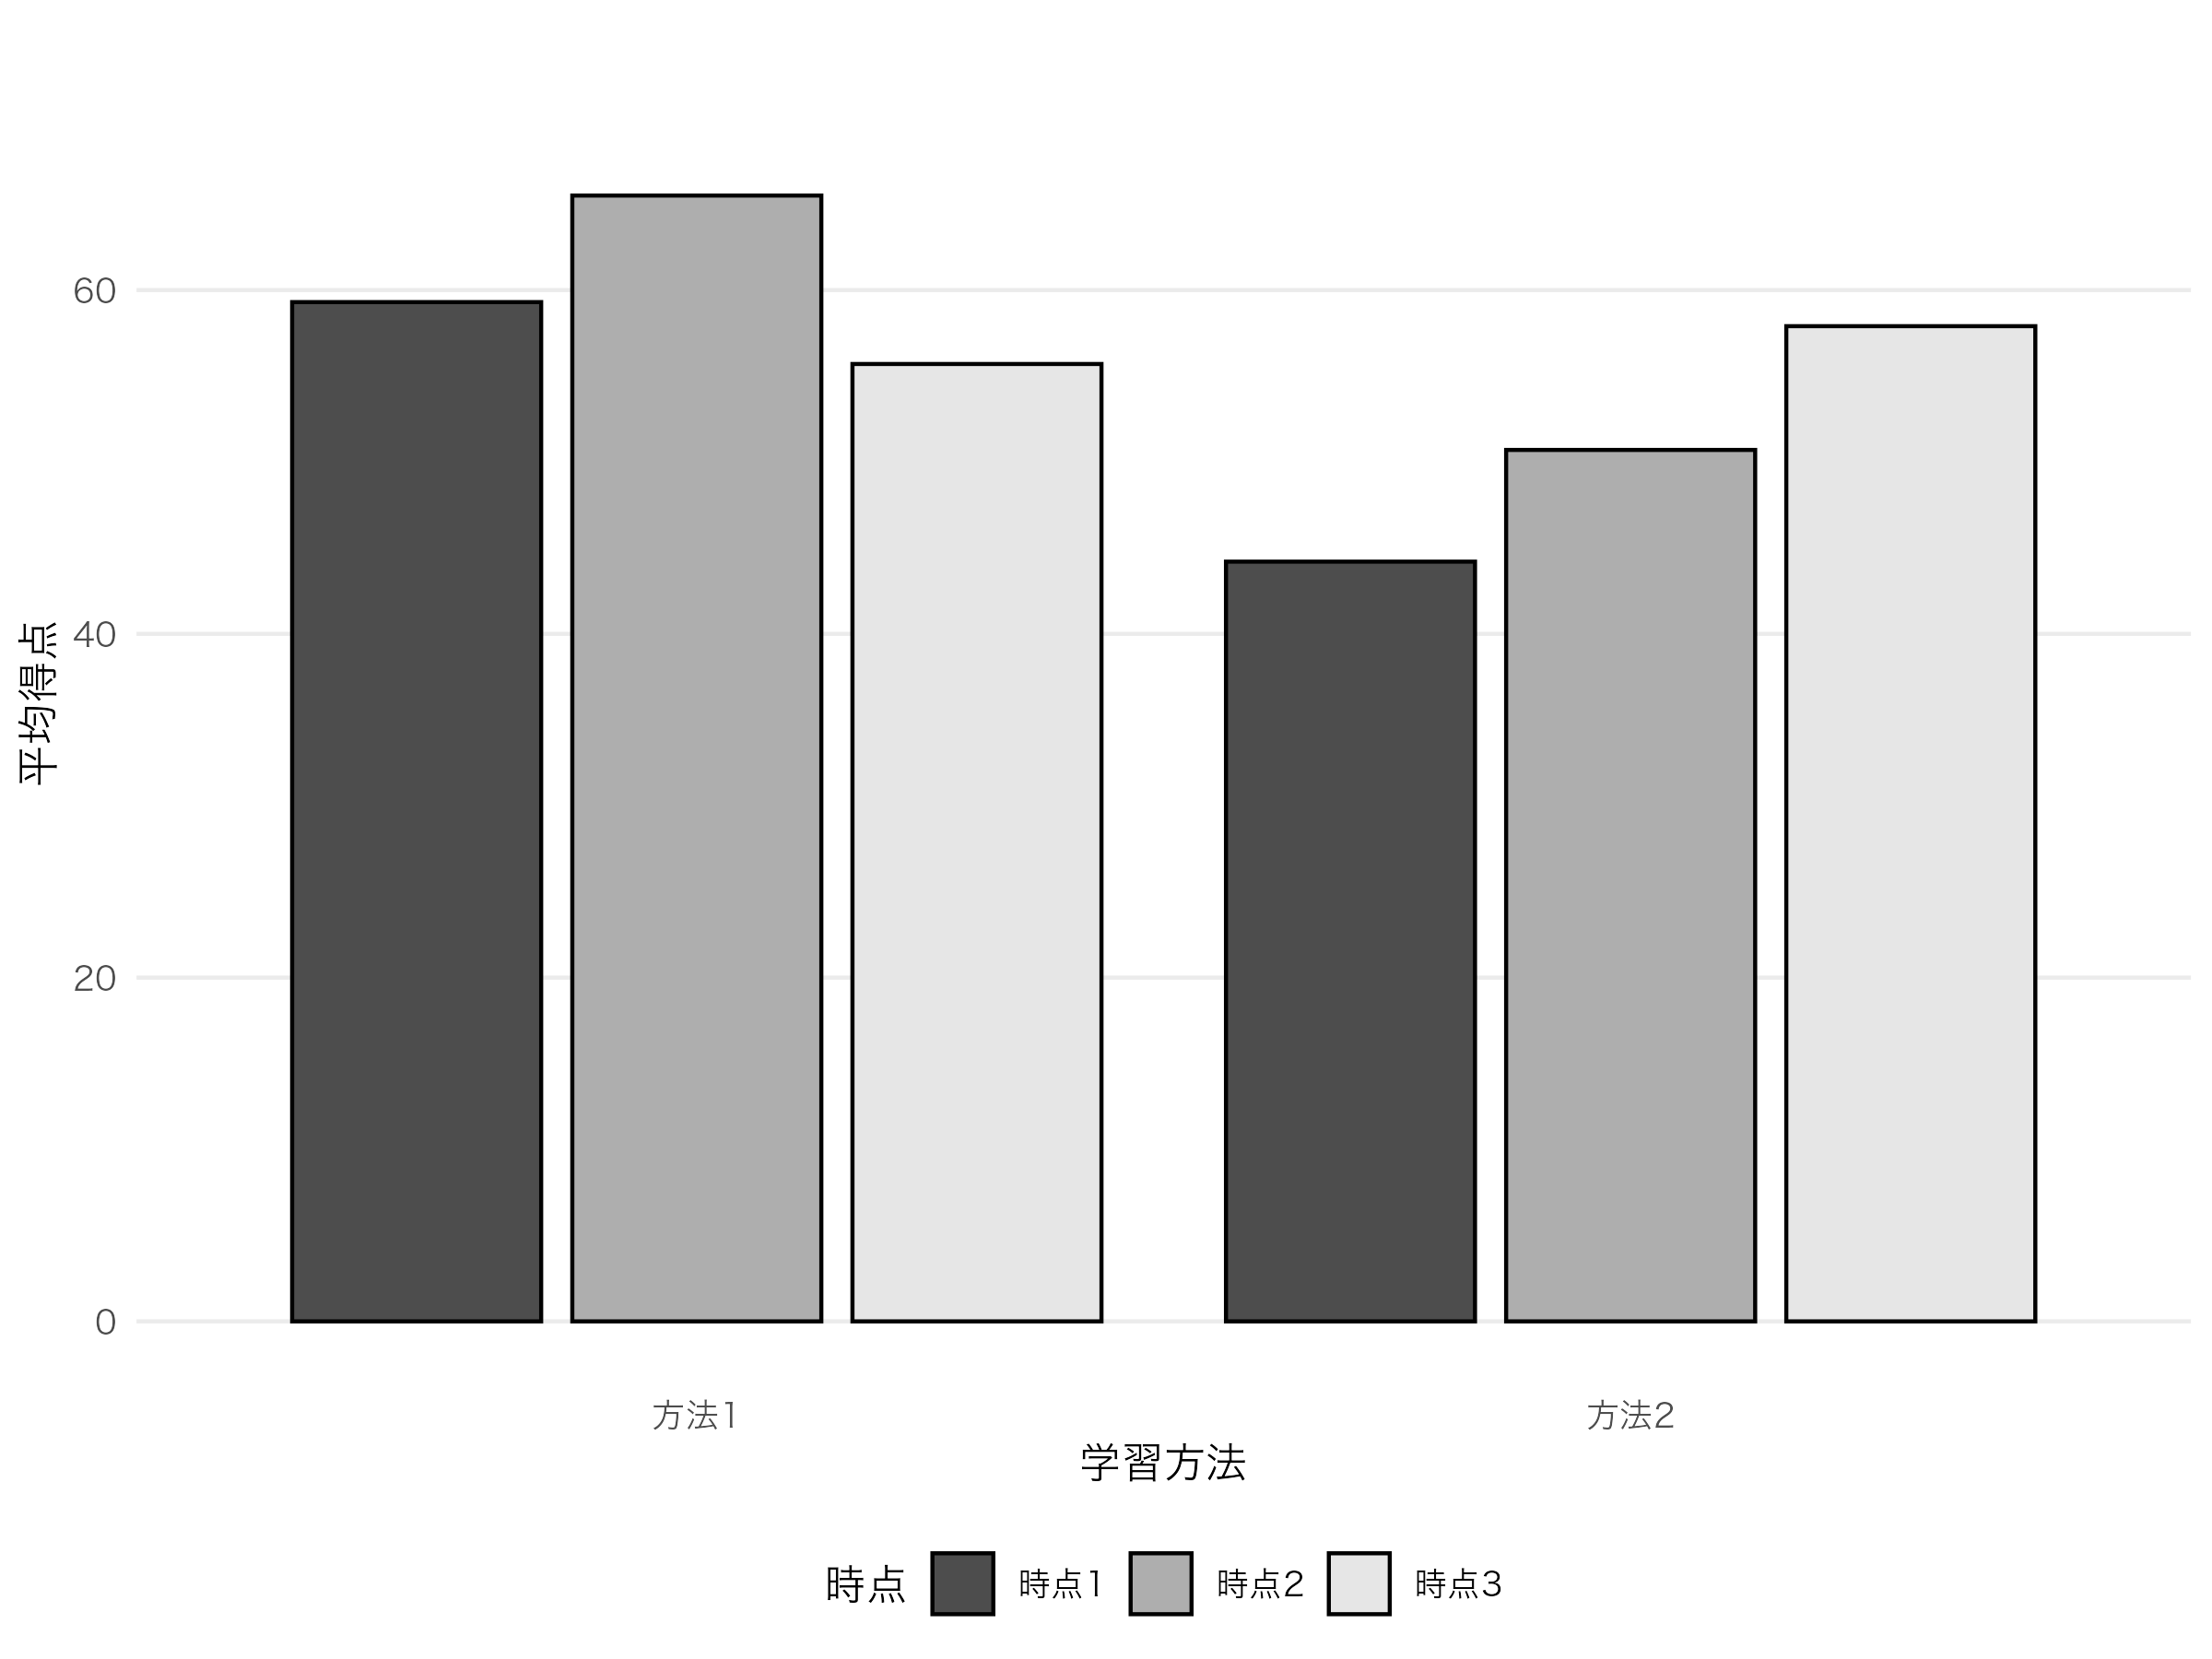
\includegraphics[keepaspectratio,width=0.8\linewidth]{figures/22_Within_R/method_by_time_barplot.png}
  \caption{二要因被験者内デザインのデータの可視化}
  \label{fig:22_02}
\end{figure}

平方和の分解は少しややこしい話になるので付録に回し，とりあえずこのデータをRに入力して，\verb|anovakun|で分析してみましょう。ポイントは，要因デザインを\verb|"sAB"|と入力するところと，A,Bそれぞれの水準数を2,3と指定するところです。また，球状性の仮定が破れている可能性を考えて，Greenhouse-Geisserの補正をかけるために\verb|gg=T|のオプションを追加してあります。コードは次のようになります(\texttt{code:\ref{code:22_03}})。

\begin{lstlisting}[language=c++,label={code:22_03},caption={二要因内$\times$内デザインのデータと分析}]
dat <- data.frame(
  id = c("A", "B", "C", "D", "E", "F", "G", "H", "I", "J"),
  m1_t1 = c(47, 60, 79, 54, 55, 84, 63, 41, 53, 57),
  m1_t2 = c(90, 71, 83, 41, 41, 103, 74, 34, 65, 53),
  m1_t3 = c(44, 63, 48, 39, 58, 20, 96, 62, 44, 83),
  m2_t1 = c(38, 39, 60, 49, 45, 62, 46, 28, 35, 40),
  m2_t2 = c(55, 49, 47, 63, 49, 58, 48, 30, 61, 47),
  m2_t3 = c(52, 59, 50, 63, 54, 56, 57, 64, 52, 72)
)

anovakun(dat[, -1], "sAB", 2, 3, eps = T, gg = T)
\end{lstlisting}

今回も滔々と結果が出てきますが，落ち着いて順番にみていきましょう。まずは球状性の仮定のチェックです(出力\ref{RS:out22_04})。

\begin{Rscreen}{下位検定の出力}{out22_04}
\begin{verbatim}
[ sAB-Type Design ]

This output was generated by anovakun 4.8.9 under R version 4.5.2.
It was executed on Tue Nov  4 16:40:26 2025.

 
<< DESCRIPTIVE STATISTICS >>

--------------------------------
  A   B   n     Mean     S.D. 
--------------------------------
 a1  b1  10  59.3000  13.2920 
 a1  b2  10  65.5000  23.0085 
 a1  b3  10  55.7000  21.9952 
 a2  b1  10  44.2000  10.6646 
 a2  b2  10  50.7000   9.4169 
 a2  b3  10  57.9000   6.7897 
--------------------------------


<< SPHERICITY INDICES >>

== Mendoza's Multisample Sphericity Test and Epsilons ==

-------------------------------------------------------------------------
 Effect  Lambda  approx.Chi  df      p         LB     GG     HF     CM 
-------------------------------------------------------------------------
 Global  0.0000     33.8813  14 0.0032 **  0.2000 0.3995 0.5134 0.4455 
      A  1.0000     -0.0000   0            1.0000 1.0000 1.0000 1.0000 
      B  0.0537      5.1974   2 0.0744 +   0.5000 0.6767 0.7542 0.6545 
  A x B  0.1145      3.8528   2 0.1457 ns  0.5000 0.7235 0.8255 0.7163 
-------------------------------------------------------------------------
                              LB = lower.bound, GG = Greenhouse-Geisser
                             HF = Huynh-Feldt-Lecoutre, CM = Chi-Muller
\end{verbatim}
\end{Rscreen}

今回，グローバルな球状性の検定が$p=0.0032$で有意になっています。つまり，球状性の仮定が破れている，と判断せざるを得ないですね。要因Aではこの問題に該当しませんが，それ以外の要因についてはこの後，Greenhouse-Geisserの補正をかけた結果が使われます。分散分析表は次のようになっています。

\begin{Rscreen}{分散分析表の出力}{out22_05}
\begin{verbatim}
<< ANOVA TABLE >>

== Adjusted by Greenhouse-Geisser's Epsilon ==

------------------------------------------------------------------------
   Source         SS    df        MS  F-ratio  p-value      epsilon^2 
------------------------------------------------------------------------
        s  2378.6833     9  264.2981                                  
------------------------------------------------------------------------
        A  1278.8167     1 1278.8167   7.1783   0.0252 *       0.0703 
    s x A  1603.3500     9  178.1500                                  
------------------------------------------------------------------------
        B   450.1000  1.35  332.5749   0.6192   0.4939 ns     -0.0177 
    s x B  6542.5667 12.18  537.1382                                  
------------------------------------------------------------------------
    A x B   980.6333  1.45  677.7204   3.6459   0.0667 +       0.0455 
s x A x B  2420.7000 13.02  185.8841                                  
------------------------------------------------------------------------
    Total 15654.8500    59  265.3364                                  
                            +p < .10, *p < .05, **p < .01, ***p < .001

\end{verbatim}
\end{Rscreen}

さてご注目。一行目の小文字sは個人差分散を表しています。これはこれまで通りですね。
そのあとは要因A,Bの主効果と交互作用(A$\times$B)の要素が出ていますが，それぞれに対応する誤差項(s x A, s x B, s x A x B)がついています。これが群内要因の分散分析のポイントです。群内要因における誤差は，個人差と要因の組み合わせによって生じるため，それぞれの要因ごとに誤差がどの程度あるかが変わるのです。群内要因の場合は「要因の効果」と「その要因に伴って生じる誤差」をセットで考えなければならない，ということですね。

詳しくみてみましょう。まず要因Aの効果の平方和(SS)は1278.8167で，対応する誤差項s x Aの平方和は1603.3500です。要因Aは2水準(m1,m2)ですから自由度(df)は1で，要因Aに伴って生じる個人差の自由度は9($=(10-1)\times(2-1)$)となっています。平均平方(MS)はSSをdfで割ったものですから，それぞれ1278.8167と178.1500になります。これらを使って$F$値を計算すると，$F=1278.8167/178.1500=7.1783$となり，対応する$p$値は0.0252で有意です。効果量$\varepsilon^2=0.0703$も計算されています。

次に要因Bですが，平方和が450.1000，対応する誤差項s x Bの平方和が6542.5667です。要因Bは3水準(t1,t2,t3)ですから自由度は2で，要因Bに伴って生じる個人差の自由度は18($=(10-1)\times(3-1)$)となっています。ただし今回は球状性の仮定が破れている可能性があるため，Greenhouse-Geisserの補正(0.6767)をかけた自由度1.35と12.18が使われています。平均平方はそれぞれ332.5749と537.1382で，$F$値は0.6192，対応する$p$値は0.4939で有意ではありません。効果量$\varepsilon^2=-0.0177$も計算されています\footnote{二乗した値がマイナスになるのはおかしいのですが，ここは有意ではないところですので不適切な値になったと思われます。}。

最後に交互作用A$\times$Bですが，平方和が980.6333，対応する誤差項s x A x Bの平方和が2420.7000です。交互作用の自由度は2で，要因A$\times$Bに伴って生じる個人差の自由度は18($=(10-1)\times(2-1)\times(3-1)$)となっています。こちらもGreenhouse-Geisserの補正(0.7235)をかけた自由度1.45と13.02が使われています。平均平方はそれぞれ677.7204と185.8841で，$F$値は3.6459，対応する$p$値は0.0667で有意水準0.05では有意ではありませんが，0.10では有意と考えられます。効果量$\varepsilon^2=0.0455$も計算されています。

これで，どこにどういう結果がでたかがわかりました。要因Aには有意な主効果があり，Bには有意な主効果はなく，交互作用は有意水準0.10で有意である，ということですね。

さて，要因Aは2水準ですから母平均が違うということは，m1の平均とm2の平均が違うというだけですから，事後の検定は不要です。交互作用も有意ではないのですが，\verb|anovakun|はデフォルトで10\%水準未満であれば一応検討するということで，交互作用についての事後の検定が行われるようになります。

この後に続く事後の検定結果を見る前に，可視化してパターンをみておきましょう。 図\ref{fig:22_03}に示します。

\begin{figure}
  \centering
  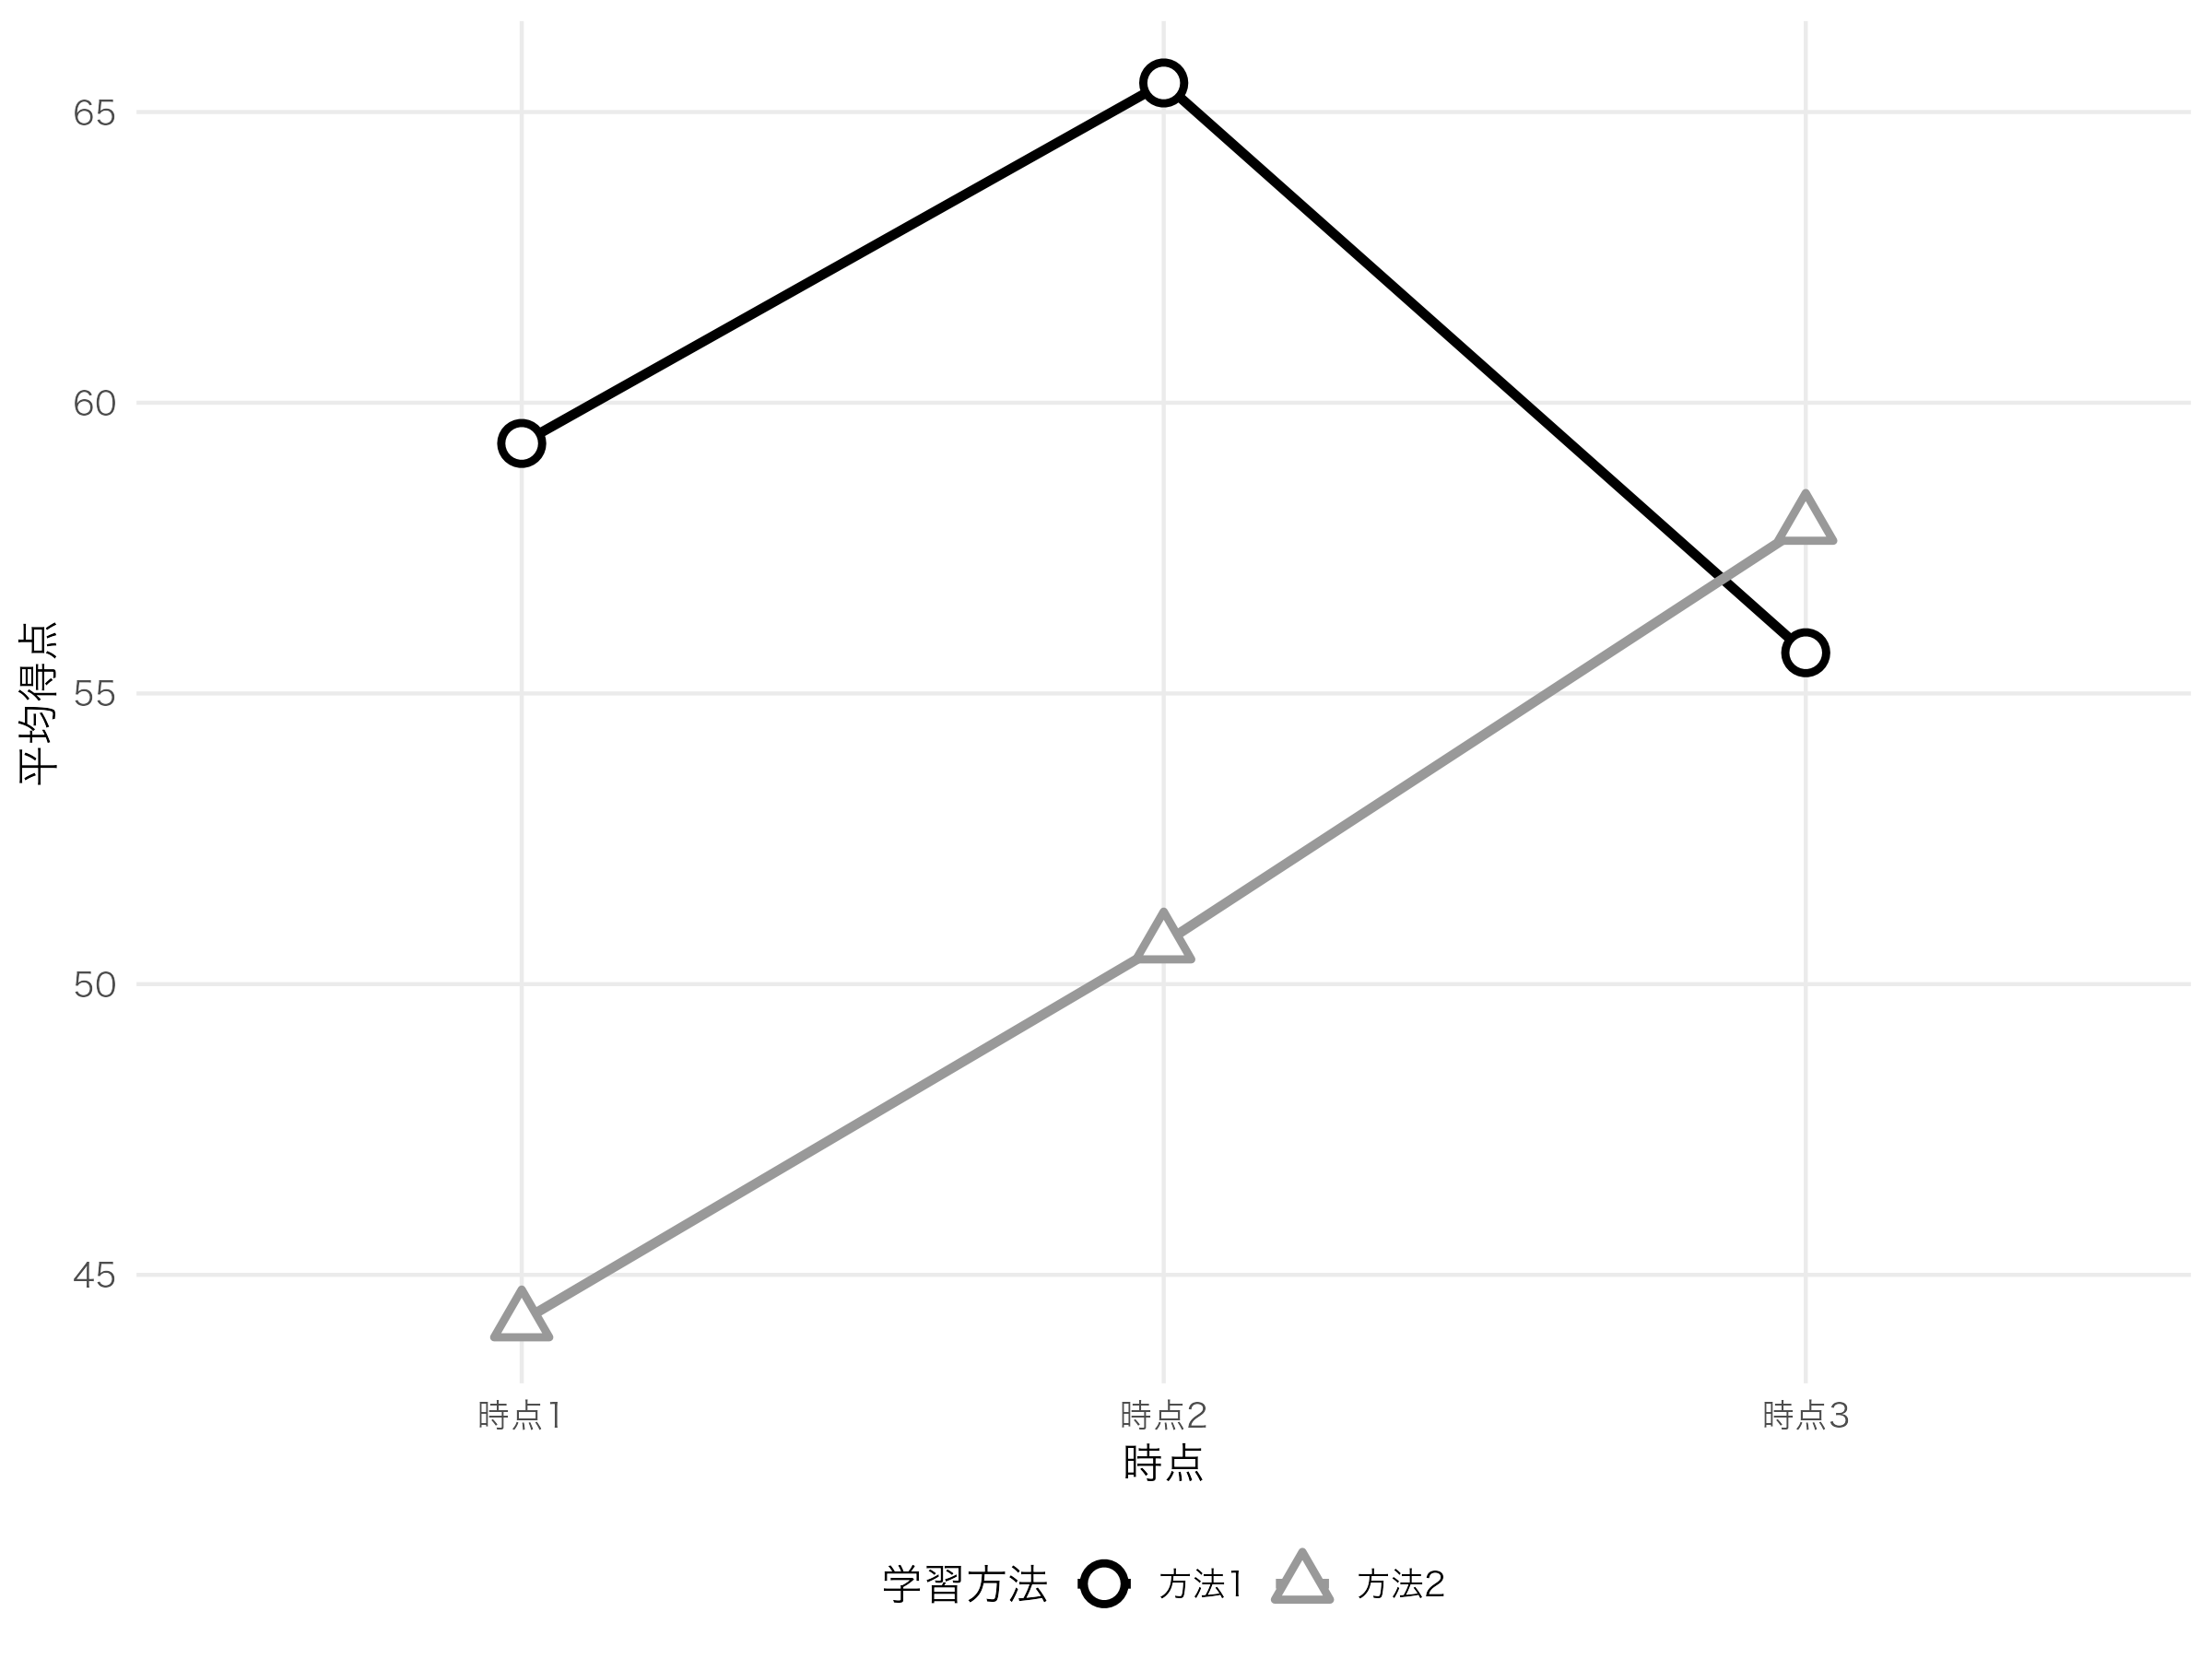
\includegraphics[keepaspectratio,width=0.8\linewidth]{figures/22_Within_R/interaction_plot.png}
  \caption{二要因被験者内デザインの交互作用の可視化}
  \label{fig:22_03}
\end{figure}


\section{単純効果の分散分析表の分割}

交互作用を細かく見る方法として，\keyterm{単純効果}{たんじゅんこうか}{simple effect}の検定があります。たとえば，図\ref{fig:22_03}を見ると，t1のときにm1とm2の差が大きく，t2,t3のときには差が小さくなっているように見えます。このような場合，t1のときにm1とm2の差が有意であるかどうかを調べることができます。これが単純効果の検定です。同様に，m1のときにt1,t2,t3の間に差があるかどうかも調べることができます。

単純効果を検定する際は，元のデータを見たいところに合わせて抽出し，小さいデータセットを作ってミニ分散分析を行う，というような形で行います。\verb|anovakun|は自動的にこれらの結果も出してくれています。出力の次の箇所を確認して下さい(出力\ref{RS:out22_06})。

\begin{Rscreen}{単純効果の出力}{out22_06}
\begin{verbatim}
<< POST ANALYSES >>

< SIMPLE EFFECTS for "A x B" INTERACTION >

--------------------------------------------------------------------------
  Effect  Lambda  approx.Chi  df      p         LB     GG     HF     CM 
--------------------------------------------------------------------------
 A at b1  1.0000     -0.0000   0            1.0000 1.0000 1.0000 1.0000 
 A at b2  1.0000     -0.0000   0            1.0000 1.0000 1.0000 1.0000 
 A at b3  1.0000     -0.0000   0            1.0000 1.0000 1.0000 1.0000 
 B at a1  0.0274      6.3967   2 0.0408 *   0.5000 0.6450 0.7068 0.6134 
 B at a2  0.6628      0.7312   2 0.6938 ns  0.5000 0.9197 1.1447 0.9933 
--------------------------------------------------------------------------
                               LB = lower.bound, GG = Greenhouse-Geisser
                              HF = Huynh-Feldt-Lecoutre, CM = Chi-Muller

-------------------------------------------------------------------------
     Source        SS    df        MS  F-ratio  p-value      epsilon^2 
-------------------------------------------------------------------------
    A at b1 1140.0500     1 1140.0500  72.5376   0.0000 ***     0.2995 
s x A at b1  141.4500     9   15.7167                                  
-------------------------------------------------------------------------
    A at b2 1095.2000     1 1095.2000   4.7714   0.0568 +       0.1300 
s x A at b2 2065.8000     9  229.5333                                  
-------------------------------------------------------------------------
    A at b3   24.2000     1   24.2000   0.1199   0.7371 ns     -0.0371 
s x A at b3 1816.8000     9  201.8667                                  
-------------------------------------------------------------------------
    B at a1  491.4667  1.29  381.0058   0.5935   0.4978 ns     -0.0301 
s x B at a1 7453.2000 11.61  642.0041                                  
-------------------------------------------------------------------------
    B at a2  939.2667  1.84  510.6523   5.5980   0.0155 *       0.2429 
s x B at a2 1510.0667 16.55   91.2200                                  
-------------------------------------------------------------------------
                             +p < .10, *p < .05, **p < .01, ***p < .001
\end{verbatim}
\end{Rscreen}

まずは，単純効果の球状性の検定結果が示されています。要因Aの各水準における要因Bの単純効果，および要因Bの各水準における要因Aの単純効果について，球状性の検定が行われています。bの各水準におけるAの効果は(2水準しかないので)球状性うんぬんの話ではないですが，aの各水準におけるBの効果については，a1水準について$p=0.0408$で有意になっています。つまり，a1水準のことを考えるときは，球状性の仮定が破れている可能性がある，ということになります。したがって，この後のa1水準におけるBの単純効果の検定では，Greenhouse-Geisserの補正がかけられた結果が使われます。

以下は単純効果の分散分析表になります。
\subsection{$\mathrm{A}\ \mathrm{at}\ \mathrm{b}_1$の単純効果}

まずは\verb|A at b1|と書かれている箇所，つまり$\mathrm{b}_1$（t1）の水準における$\mathrm{A}$（方法）の単純効果を検定することを考えましょう。
やっていることは，m1\_t1とm2\_t1のデータだけを使用した分散分析と同じです。つまり表\ref{tbl:22_03a}のようなデータに対して分散分析をしているようなものです。

\begin{table}[ht]
\centering
\begin{tabular}{lrr}
  \hline
id & m1\_t1 & m2\_t1 \\
  \hline
A & 47 & 38 \\
B & 60 & 39 \\
C & 79 & 60 \\
D & 54 & 49 \\
E & 55 & 45 \\
F & 84 & 62 \\
G & 63 & 46 \\
H & 41 & 28 \\
I & 53 & 35 \\
J & 57 & 40 \\
  \hline
\end{tabular}
\caption{$\mathrm{A}\ \mathrm{at}\ \mathrm{b}_1$の単純効果検定用データ（t1のみ）}
\label{tbl:22_03a}
\end{table}

実際にこのデータに対して，一要因の群内計画の分散分析をやってみることができます。Rでは次のように実行します。

\begin{lstlisting}[language=c++,label={code:22_04},caption={A at b1の単純効果検定}]
SimpleEffectA_at_b1 <- dat[, c(2, 5)]
anovakun(SimpleEffectA_at_b1, "sA", 2)
\end{lstlisting}
これで出力されるのは，ここの表に含まれているものと同じです(出力\ref{RS:out22_07})。

\begin{Rscreen}{ミニデータの分散分析結果}{out22_07}
\begin{verbatim}
  << ANOVA TABLE >>

-----------------------------------------------------------
 Source         SS  df         MS  F-ratio  p-value      
-----------------------------------------------------------
      s  2472.2500   9   274.6944                        
-----------------------------------------------------------
      A  1140.0500   1  1140.0500  72.5376   0.0000 ***  
  s x A   141.4500   9    15.7167                        
-----------------------------------------------------------
  Total  3753.7500  19   197.5658                        
               +p < .10, *p < .05, **p < .01, ***p < .001
\end{verbatim}
\end{Rscreen}

ここでは有意であるという結果になっていますので，t1のときにはm1とm2の間に有意な差がある，ということがわかります。図\ref{fig:22_03}を見ても，t1のときにm1とm2の差が大きいことがわかりますね。

\subsection{$\mathrm{B}\ \mathrm{at}\ \mathrm{a}_2$の単純効果}

以下同様の分割・分析が行われており，もう一つ有意なマークがついているのが，\verb|B at a2|の箇所です。これはm2のときにt1,t2,t3の間に差があるかどうかを調べる単純効果の検定です。こちらも同様にミニデータを作って分散分析を行うことができます(表\ref{tbl:22_04b})。

\begin{table}[ht]
\centering
\begin{tabular}{lrrr}
  \hline
id & m2\_t1 & m2\_t2 & m2\_t3 \\
  \hline
A & 38 & 55 & 52 \\
B & 39 & 49 & 59 \\
C & 60 & 47 & 50 \\
D & 49 & 63 & 63 \\
E & 45 & 49 & 54 \\
F & 62 & 58 & 56 \\
G & 46 & 48 & 57 \\
H & 28 & 30 & 64 \\
I & 35 & 61 & 52 \\
J & 40 & 47 & 72 \\
  \hline
\end{tabular}
\caption{$\mathrm{B}\ \mathrm{at}\ \mathrm{a}_2$の単純効果検定用データ（m2のみ）}
\label{tbl:22_04b}
\end{table}

このデータに対して，一要因の群内計画の分散分析を行います。Rでは次のように実行します。
もっとも，同じ結果はすでに全体の分析結果の中に含まれているので，あえて実行する必要はありません。ここでは全体出力の最後のところを抜き出してみました(出力\ref{RS:out22_08})。

これはa2水準における要因Bの効果を検証しているところで，これが有意($F(1.84,16.55)=5.5980,p=0.0155,\varepsilon^2=0.2429$)だったのですから，t1,t2,t3間のどこかに差があったわけです。どこに差があったのかがわからないので，さらに事後の検定が行われています。それが\verb|< MULTIPLE COMPARISON for "B at a2" >|のところなのです。

\begin{lstlisting}[language=c++,label={code:22_05},caption={B at a2の単純効果検定}]
SimpleEffectB_at_a2 <- dat[, c(5, 6, 7)]
anovakun(SimpleEffectB_at_a2, "sA", 3, gg = T)
\end{lstlisting}

\begin{Rscreen}{ミニデータの分散分析結果}{out22_08}
\begin{verbatim}

< MULTIPLE COMPARISON for "B at a2" >

== Shaffer's Modified Sequentially Rejective Bonferroni Procedure ==
== The factor < B at a2 > is analysed as dependent means. == 
== Alpha level is 0.05. == 
 
-----------------------------------------------------------
  Pair      Diff  t-value  df       p   adj.p            
-----------------------------------------------------------
 b1-b3  -13.7000   3.0119   9  0.0147  0.0440  b1 < b3 * 
 b1-b2   -6.5000   1.8622   9  0.0955  0.0955  b1 = b2   
 b2-b3   -7.2000   1.7230   9  0.1190  0.1190  b2 = b3   
-----------------------------------------------------------
\end{verbatim}
\end{Rscreen}

これを見ると，t1とt3のペアが有意であることがわかります。つまり，m2のときにはt1とt3の間に有意な差があった，ということですね。図\ref{fig:22_03}を見ても，m2のときにt1とt3の差が大きいことがわかります。


\section{分散分析のまとめ}
長い道のりでしたが，これで一通り分散分析の説明は終わりです。最後に，分散分析のポイントをまとめておきましょう。
\begin{itemize}
  \item 分散分析は，データのばらつきを要因ごとに分解し，その要因がデータに与える影響を検証する手法である。
  \item 「分散」分析という名前がついているが，目的は平均値の比較である。「分散」という名前がついているのは，比較に際して要因が引き起こすばらつき(分散)と，説明できないばらつき(分散)を比較するからである。
  \item 分散と分散の比較の確率分布は$F$分布である。
  \item 群間計画では，各要因の効果と全体の誤差項を使って$F$値を計算する。
  \item 群内計画では，各要因の効果とそれに伴って生じる誤差を使って$F$値を計算する。
  \item 要因が2つ以上になると，組み合わせの効果すなわち交互作用も検証する。
  \item 水準が3つ以上になると，どの水準間で差があるのかを調べるために事後の検定を行う。
\end{itemize}

最後の内$\times$内デザインでみたように，分散分析の事後の検定(交互作用の検定)では，分散分析表をさらに分割して，ミニ分散分析を行うことで検証を行っていきます。これが分散分析の基本的な考え方です。

また水準が多い場合は，タイプ1エラーが起きる確率($\alpha$,有意水準に同じ)を制御するために，様々な補正をかけた分析を行います。TukeyのHSD法や修正Bonferroni法などがそれです。これらの方法も\verb|anovakun|で自動的に行うことができます。

分散分析は，多様なデザインに対応できる強力な判断技術です。数字の計算は困難に見えるかもしれませんが，難しい(difficult)のではなく，簡単(easy)な要素が複雑(complex)に絡み合っているのでそう見えるだけなのです。実際，分散分析は手計算でも効果や誤差を計算できるわけです。それを統計パッケージRが代わってくれるので，結果はますます簡単に得られます。

ユーザである我々に必要なのは，正しく結果を読み取り，解釈する能力です。あるいは，分散分析に落とし込めば良い問題を見つける，分散分析で解決できるように実験をデザインする能力です。それは心理学を学んでいくなかで，自然と身につくでしょう。

ただ残念ながら，分散分析はレガシーといいますか，古典的な技術です。進んだ心理学の研究では，分散分析をより発展させたモデル，線形モデルをより展開したモデルが使われています。次回からは線形モデルを拡張するのに必要な，確率分布と線形モデルの合体について学んでいきましょう。

\section{課題}
二要因群内デザインのデータをそのまま使います。ただし，今回は要因Aが群間要因だったと考えてください。つまり，方法1と方法2で別々の被験者群が割り当てられたと考えます。この場合の分散分析をRで行い，結果を解釈してください。参考までに，データを生成するコードの例をコード\ref{code:22_06}に示します。

\begin{lstlisting}[language=c++,label={code:22_06},caption={二要因混合デザインのデータと分析}]
# m1グループのデータ
dat_m1 <- data.frame(
  group = rep("m1", 10),
  t1 = dat$m1_t1[1:5],
  t2 = dat$m1_t2[1:5],
  t3 = dat$m1_t3[1:5]
)

# m2グループのデータ
dat_m2 <- data.frame(
  group = rep("m2", 10),
  t1 = dat$m2_t1[6:10],
  t2 = dat$m2_t2[6:10],
  t3 = dat$m2_t3[6:10]
)

# 2つのグループを結合
dat_between <- rbind(dat_m1, dat_m2)
\end{lstlisting}

\section{補遺；群内計画の平方和の分解}
二要因群間要因の分散分析では，平方和の分解を行いました。今回，群内要因のときはそれを行わずにいきなり\verb|anovakun|に計算させました。その理由はなんといっても複雑だからです。そしてその複雑な計算をひとつひとつ説明しても，レガシーとなった技術の細部を掘り返すようで，あまり意味がないかもしれません。

しかし，だからこそマニアックなあなたのために，説明を追加しておこうと思います。知的なエッセイとして読んでいただいても結構ですし，足し算と掛け算だけでできる算数パズルだとおもって一緒に計算してみていただいても結構です。

さあ，楽しみましょう！

\subsection{個人差の計算}
まずは個人差です。データは一行が一人分を表していますから，各行の平均値を計算することで「その人の平均」を見ることができ，それが全体平均からどれぐらい隔たっているかで，個人差の効果を計算することができます。計算プロセスを表\ref{tbl:22_05}に示します。

\begin{table}[ht]
\centering
\begin{tabular}{lrrrrr}
  \hline
id & 平均 & 効果 & 効果二乗 & 要素数 & SS寄与 \\
  \hline
A & 54.33 & -1.22 & 1.48 & 6 & 8.88 \\
B & 56.83 & 1.28 & 1.65 & 6 & 9.88 \\
C & 61.17 & 5.62 & 31.55 & 6 & 189.28 \\
D & 51.50 & -4.05 & 16.40 & 6 & 98.41 \\
E & 50.33 & -5.22 & 27.21 & 6 & 163.28 \\
F & 63.83 & 8.28 & 68.61 & 6 & 411.68 \\
G & 64.00 & 8.45 & 71.40 & 6 & 428.42 \\
H & 43.17 & -12.38 & 153.35 & 6 & 920.08 \\
I & 51.67 & -3.88 & 15.08 & 6 & 90.48 \\
J & 58.67 & 3.12 & 9.71 & 6 & 58.28 \\
  \hline
合計 &  &  &  &  & 2378.68 \\
   \hline
\end{tabular}
\caption{個人差の計算}
\label{tbl:22_05}
\end{table}

一行目，$A$さんのデータを見てみましょう。$A$さんの各条件における得点は，47,90,44,38,55,52で，平均は54.33になります。全体平均が55.55でしたから，効果は$54.33-55.55=-1.22$となります。これがこの人の効果です。この効果を二乗すると1.48になり，これが一行分・6ケース全てにあらわれていますから，平方和に寄与するのは$1.48\times 6=8.88$と考えられます。これを全員分計算して，最後に合計を出すと2378.68となり，個人差の平方和(SS)が得られます。分散分析表でも最初にこの数字が出ていましたね。

\subsection{主効果の計算}
今度は要因ごとの効果です。要因Aと要因Bの主効果を計算してみましょう。要因Aは2水準，Bは3水準ですから，それぞれの水準ごとに平均を計算し，全体平均からどれぐらい隔たっているかを見ます。表\ref{tbl:22_06}に示します。
\begin{table}[ht]
\centering
\begin{tabular}{lrrrc|r|r}
  \hline
水準 & 平均 & 効果 & 効果二乗 & 要素数 & SS寄与 & 合計\\
  \hline
m1 & 60.17 & 4.62 & 21.31 & 30 & 639.41 & \multirow{2}{*}{1278.82}\\
m2 & 50.93 & -4.62 & 21.31 & 30 & 639.41 & \\\hline
t1 & 51.75 & -3.80 & 14.44 & 20 & 288.80 & \multirow{3}{*}{450.10}\\
t2 & 58.10 & 2.55 & 6.50 & 20 & 130.05 & \\
t3 & 56.80 & 1.25 & 1.56 & 20 & 31.25 & \\\hline
\end{tabular}
\caption{主効果の計算}
\label{tbl:22_06}
\end{table}

ここでも，一行目，m1水準を見てみましょう。m1水準の平均は60.17で，全体平均55.55からの効果は$60.17-55.55=4.62$となります。この効果を二乗すると21.31になり，m1水準には30ケース(10人$\times$3水準)ありますから，平方和に寄与するのは$21.31\times 30=639.41$と考えられます。これをm2水準についても同様に計算し，合計すると要因Aの平方和1278.82が得られます。要因Bについても同様に計算し，平方和450.10が得られます。分散分析表にもこの数字がありましたね！

\subsection{交互作用の計算}
今度は交互作用です。交互作用は組み合わせの水準ごとに平均値を出します。
例えばm1t1の水準の平均は59.30です。全体平均は55.55，これに要因Aのm1効果4.62と要因Bのt1効果-3.80を足し合わせると，予測平均は$55.55+4.62-3.80=56.37$となります。交互作用がなければ56.37になるはずですが，実際の平均は59.30ですから，逆算すると交互作用の効果は，$59.30-56.37=2.93$だったことがわかります。この効果を二乗すると8.60になり，m1t1水準には10ケース(10人$\times$1水準)ありますから，平方和に寄与するのは$8.60\times 10=86.04$と考えられます。これを全ての組み合わせ水準について計算し，最後に合計すると交互作用の平方和980.63が得られます。計算のステップを表\ref{tbl:22_07}に示します。

\begin{table}[ht]
\centering
\begin{tabular}{lrrrrrr}
  \hline
セル & 観測平均 & 予測平均 & 交互作用効果 & 効果二乗 & 要素数 & SS寄与 \\
  \hline
m1t1 & 59.30 & 56.37 & 2.93 & 8.60 & 10 & 86.04 \\
  m1t2 & 65.50 & 62.72 & 2.78 & 7.75 & 10 & 77.47 \\
  m1t3 & 55.70 & 61.42 & -5.72 & 32.68 & 10 & 326.80 \\
  m2t1 & 44.20 & 47.13 & -2.93 & 8.60 & 10 & 86.04 \\
  m2t2 & 50.70 & 53.48 & -2.78 & 7.75 & 10 & 77.47 \\
  m2t3 & 57.90 & 52.18 & 5.72 & 32.68 & 10 & 326.80 \\
  \hline
  合計 &  &  &  &  &  & 980.63 \\
   \hline
\end{tabular}
\caption{交互作用の計算}
\label{tbl:22_07}
\end{table}

\subsection{要因Aに伴って生じる残差}
群内計画がややこしいのはここからです！残差が要因に伴って生じる，という考え方をする必要があります。要因Aに伴って生じる残差は，要因Bのそれとは違うんだぞ，ということを考えます。まずBの3つの水準を平均した値を計算しましょう。表\ref{tbl:22_08}に示します。

\begin{table}[ht]
\centering
\begin{tabular}{lrr}
  \hline
id & m1 & m2 \\
  \hline
A & 60.33 & 48.33 \\
  B & 64.67 & 49.00 \\
  C & 70.00 & 52.33 \\
  D & 44.67 & 58.33 \\
  E & 51.33 & 49.33 \\
  F & 69.00 & 58.67 \\
  G & 77.67 & 50.33 \\
  H & 45.67 & 40.67 \\
  I & 54.00 & 49.33 \\
  J & 64.33 & 53.00 \\
   \hline
\end{tabular}
\caption{各被験者の要因A水準別平均}
\label{tbl:22_08}
\end{table}

これは要因Bの影響を取り除いた(要因Bで平均化した)要因A水準別の各被験者の平均値です。
例えばAさんのm1水準の値を考えてみましょう。Aさんのm1水準の各条件における得点は，47,90,44で，平均は60.33になります。これが要因Bの影響を取り除いたときの，Aさんのm1水準における得点です。
全体平均55.55，Aさんの個人差は-1.22，m1水準の効果は4.62ですから，予測平均は$55.55-1.22+4.62=58.95$です。いっぽう，実際の平均は60.33ですから，残差は$60.33-58.95=1.38$となります。これが要因Bに関係のない，要因Aに伴って生じる残差です。

この残差を二乗すると1.91になり，m1水準には3ケース(3つの要因B水準)ありますから，平方和に寄与するのは$1.91\times 3=5.74$と考えられます。これを全ての組み合わせ水準について計算し，最後に合計すると要因Aに伴う残差の平方和1603.35が得られます。計算のステップを表\ref{tbl:22_09}に示します。

\begin{table}[ht]
\centering
\small
\begin{tabular}{llrrrrrrrr}
  \hline
id & A水準 & 観測平均 & 個人差効果 & A効果 & 予測平均 & 残差 & 残差二乗 & 要素数 & SS寄与 \\
  \hline
A & m1 & 60.33 & -1.22 & 4.62 & 58.95 & 1.38 & 1.91 & 3 & 5.74 \\
  A & m2 & 48.33 & -1.22 & -4.62 & 49.72 & -1.38 & 1.91 & 3 & 5.74 \\
  B & m1 & 64.67 & 1.28 & 4.62 & 61.45 & 3.22 & 10.35 & 3 & 31.04 \\
  B & m2 & 49.00 & 1.28 & -4.62 & 52.22 & -3.22 & 10.35 & 3 & 31.04 \\
  C & m1 & 70.00 & 5.62 & 4.62 & 65.78 & 4.22 & 17.78 & 3 & 53.34 \\
  C & m2 & 52.33 & 5.62 & -4.62 & 56.55 & -4.22 & 17.78 & 3 & 53.34 \\
  D & m1 & 44.67 & -4.05 & 4.62 & 56.12 & -11.45 & 131.10 & 3 & 393.31 \\
  D & m2 & 58.33 & -4.05 & -4.62 & 46.88 & 11.45 & 131.10 & 3 & 393.31 \\
  E & m1 & 51.33 & -5.22 & 4.62 & 54.95 & -3.62 & 13.08 & 3 & 39.24 \\
  E & m2 & 49.33 & -5.22 & -4.62 & 45.72 & 3.62 & 13.08 & 3 & 39.24 \\
  F & m1 & 69.00 & 8.28 & 4.62 & 68.45 & 0.55 & 0.30 & 3 & 0.91 \\
  F & m2 & 58.67 & 8.28 & -4.62 & 59.22 & -0.55 & 0.30 & 3 & 0.91 \\
  G & m1 & 77.67 & 8.45 & 4.62 & 68.62 & 9.05 & 81.90 & 3 & 245.71 \\
  G & m2 & 50.33 & 8.45 & -4.62 & 59.38 & -9.05 & 81.90 & 3 & 245.71 \\
  H & m1 & 45.67 & -12.38 & 4.62 & 47.78 & -2.12 & 4.48 & 3 & 13.44 \\
  H & m2 & 40.67 & -12.38 & -4.62 & 38.55 & 2.12 & 4.48 & 3 & 13.44 \\
  I & m1 & 54.00 & -3.88 & 4.62 & 56.28 & -2.28 & 5.21 & 3 & 15.64 \\
  I & m2 & 49.33 & -3.88 & -4.62 & 47.05 & 2.28 & 5.21 & 3 & 15.64 \\
  J & m1 & 64.33 & 3.12 & 4.62 & 63.28 & 1.05 & 1.10 & 3 & 3.31 \\
  J & m2 & 53.00 & 3.12 & -4.62 & 54.05 & -1.05 & 1.10 & 3 & 3.31 \\
  \hline
  合計 &  &  &  &  &  &  &  &  & 1603.35 \\
   \hline
\end{tabular}
\caption{要因Aに伴う残差（s×A）の計算}
\label{tbl:22_09}
\end{table}

\subsection{要因Bに伴って生じる残差}
今度は要因Bに伴って生じる残差です。要因Bに伴って生じる残差は，要因Aのそれとは違うと考えますから，要因Aの水準を潰して平均化したデータを考えましょう。これを表\ref{tbl:22_10}に示します。
\begin{table}[ht]
\centering
\begin{tabular}{lrrr}
  \hline
id & t1 & t2 & t3 \\
  \hline
A & 42.50 & 72.50 & 48.00 \\
  B & 49.50 & 60.00 & 61.00 \\
  C & 69.50 & 65.00 & 49.00 \\
  D & 51.50 & 52.00 & 51.00 \\
  E & 50.00 & 45.00 & 56.00 \\
  F & 73.00 & 80.50 & 38.00 \\
  G & 54.50 & 61.00 & 76.50 \\
  H & 34.50 & 32.00 & 63.00 \\
  I & 44.00 & 63.00 & 48.00 \\
  J & 48.50 & 50.00 & 77.50 \\
   \hline
\end{tabular}
\caption{各被験者の要因B水準別平均}
\label{tbl:22_10}
\end{table}

さて，またAさんのt1水準を考えてみましょう。Aさんのt1水準の各条件における得点は，47,38で，平均は42.50になります。これが要因Aの影響を取り除いた(要因Aで平均化した)ときの，Aさんのt1水準における得点です。
全体平均55.55，Aさんの個人差は-1.22，t1水準の効果は-3.80ですから，予測平均は$55.55-1.22-3.80=50.53$です。いっぽう，実際の平均は42.50ですから，残差は$42.50-50.53=-8.03$となります。これが要因Aに関係のない，要因Bに伴って生じる残差です。

これを二乗し，要素数(今回はAの2水準だから2)をかけると，平方和に寄与する値が得られます。これを全ての組み合わせ水準について計算し，最後に合計すると要因Bに伴う残差の平方和6542.57が得られます。計算のステップを表\ref{tbl:22_11}に示します。

\begin{table}[ht]
\centering
\small
\begin{tabular}{llrrrrrrrr}
  \hline
id & B水準 & 観測平均 & 個人差効果 & B効果 & 予測平均 & 残差 & 残差二乗 & 要素数 & SS寄与 \\
  \hline
A & t1 & 42.50 & -1.22 & -3.80 & 50.53 & -8.03 & 64.53 & 2 & 129.07 \\
  A & t2 & 72.50 & -1.22 & 2.55 & 56.88 & 15.62 & 243.88 & 2 & 487.76 \\
  A & t3 & 48.00 & -1.22 & 1.25 & 55.58 & -7.58 & 57.51 & 2 & 115.01 \\
  B & t1 & 49.50 & 1.28 & -3.80 & 53.03 & -3.53 & 12.48 & 2 & 24.97 \\
  B & t2 & 60.00 & 1.28 & 2.55 & 59.38 & 0.62 & 0.38 & 2 & 0.76 \\
  B & t3 & 61.00 & 1.28 & 1.25 & 58.08 & 2.92 & 8.51 & 2 & 17.01 \\
  C & t1 & 69.50 & 5.62 & -3.80 & 57.37 & 12.13 & 147.22 & 2 & 294.44 \\
  C & t2 & 65.00 & 5.62 & 2.55 & 63.72 & 1.28 & 1.65 & 2 & 3.29 \\
  C & t3 & 49.00 & 5.62 & 1.25 & 62.42 & -13.42 & 180.01 & 2 & 360.01 \\
  D & t1 & 51.50 & -4.05 & -3.80 & 47.70 & 3.80 & 14.44 & 2 & 28.88 \\
  D & t2 & 52.00 & -4.05 & 2.55 & 54.05 & -2.05 & 4.20 & 2 & 8.41 \\
  D & t3 & 51.00 & -4.05 & 1.25 & 52.75 & -1.75 & 3.06 & 2 & 6.12 \\
  E & t1 & 50.00 & -5.22 & -3.80 & 46.53 & 3.47 & 12.02 & 2 & 24.04 \\
  E & t2 & 45.00 & -5.22 & 2.55 & 52.88 & -7.88 & 62.15 & 2 & 124.29 \\
  E & t3 & 56.00 & -5.22 & 1.25 & 51.58 & 4.42 & 19.51 & 2 & 39.01 \\
  F & t1 & 73.00 & 8.28 & -3.80 & 60.03 & 12.97 & 168.13 & 2 & 336.27 \\
  F & t2 & 80.50 & 8.28 & 2.55 & 66.38 & 14.12 & 199.28 & 2 & 398.56 \\
  F & t3 & 38.00 & 8.28 & 1.25 & 65.08 & -27.08 & 733.51 & 2 & 1467.01 \\
  G & t1 & 54.50 & 8.45 & -3.80 & 60.20 & -5.70 & 32.49 & 2 & 64.98 \\
  G & t2 & 61.00 & 8.45 & 2.55 & 66.55 & -5.55 & 30.80 & 2 & 61.61 \\
  G & t3 & 76.50 & 8.45 & 1.25 & 65.25 & 11.25 & 126.56 & 2 & 253.12 \\
  H & t1 & 34.50 & -12.38 & -3.80 & 39.37 & -4.87 & 23.68 & 2 & 47.37 \\
  H & t2 & 32.00 & -12.38 & 2.55 & 45.72 & -13.72 & 188.15 & 2 & 376.29 \\
  H & t3 & 63.00 & -12.38 & 1.25 & 44.42 & 18.58 & 345.34 & 2 & 690.68 \\
  I & t1 & 44.00 & -3.88 & -3.80 & 47.87 & -3.87 & 14.95 & 2 & 29.90 \\
  I & t2 & 63.00 & -3.88 & 2.55 & 54.22 & 8.78 & 77.15 & 2 & 154.29 \\
  I & t3 & 48.00 & -3.88 & 1.25 & 52.92 & -4.92 & 24.17 & 2 & 48.35 \\
  J & t1 & 48.50 & 3.12 & -3.80 & 54.87 & -6.37 & 40.53 & 2 & 81.07 \\
  J & t2 & 50.00 & 3.12 & 2.55 & 61.22 & -11.22 & 125.81 & 2 & 251.63 \\
  J & t3 & 77.50 & 3.12 & 1.25 & 59.92 & 17.58 & 309.17 & 2 & 618.35 \\
  \hline
  合計 &  &  &  &  &  &  &  &  & 6542.57 \\
   \hline
\end{tabular}
\caption{要因Bに伴う残差（s×B）の計算}
\label{tbl:22_11}
\end{table}
分散分析表でみた値が出ましたね！ここまでくれば後少しです。

\subsection{交互作用に伴って生じる残差}
後少し，と言いながらこれが厄介。というのも，各セルについて考えなければならない話だからです。各セルについて，交互作用に伴って生じる残差を計算します。例えばAさんのm1t1セルを考えてみましょう。観測値は47です。個人差効果は-1.22，A効果は4.62，B効果は-3.80，交互作用効果は2.93です。さらに，m1に伴って生じるズレ(残差)が1.38，t1に伴って生じるズレ(残差)が-8.03加わります。これらを全部足し合わせると，予測値は51.43になります。実際の観測値は47ですから，残差は-4.43となります。この残差を二乗すると19.65になり，これがSSに寄与します。これを全てのセルについて計算し，最後に合計すると交互作用に伴う残差の平方和2420.70が得られます。計算のステップを表\ref{tbl:22_12}に示します。


\begin{table}[p]
\centering
\tiny
\begin{tabular}{llrrrrrrrrrrr}
  \hline
id & セル & 観測値 & 個人差 & A効果 & B効果 & AB & s$\times$A & s$\times$B & 予測 & 残差 & 残差$^2$ & SS \\
  \hline
A & m1\_t1 & 47 & -1.22 & 4.62 & -3.80 & 2.93 & 1.38 & -8.03 & 51.43 & -4.43 & 19.65 & 19.65 \\
A & m1\_t2 & 90 & -1.22 & 4.62 & 2.55 & 2.78 & 1.38 & 15.62 & 81.28 & 8.72 & 75.98 & 75.98 \\
A & m1\_t3 & 44 & -1.22 & 4.62 & 1.25 & -5.72 & 1.38 & -7.58 & 48.28 & -4.28 & 18.35 & 18.35 \\
A & m2\_t1 & 38 & -1.22 & -4.62 & -3.80 & -2.93 & -1.38 & -8.03 & 33.57 & 4.43 & 19.65 & 19.65 \\
A & m2\_t2 & 55 & -1.22 & -4.62 & 2.55 & -2.78 & -1.38 & 15.62 & 63.72 & -8.72 & 75.98 & 75.98 \\
A & m2\_t3 & 52 & -1.22 & -4.62 & 1.25 & 5.72 & -1.38 & -7.58 & 47.72 & 4.28 & 18.35 & 18.35 \\
B & m1\_t1 & 60 & 1.28 & 4.62 & -3.80 & 2.93 & 3.22 & -3.53 & 60.27 & -0.27 & 0.07 & 0.07 \\
B & m1\_t2 & 71 & 1.28 & 4.62 & 2.55 & 2.78 & 3.22 & 0.62 & 70.62 & 0.38 & 0.15 & 0.15 \\
B & m1\_t3 & 63 & 1.28 & 4.62 & 1.25 & -5.72 & 3.22 & 2.92 & 63.12 & -0.12 & 0.01 & 0.01 \\
B & m2\_t1 & 39 & 1.28 & -4.62 & -3.80 & -2.93 & -3.22 & -3.53 & 38.73 & 0.27 & 0.07 & 0.07 \\
B & m2\_t2 & 49 & 1.28 & -4.62 & 2.55 & -2.78 & -3.22 & 0.62 & 49.38 & -0.38 & 0.15 & 0.15 \\
B & m2\_t3 & 59 & 1.28 & -4.62 & 1.25 & 5.72 & -3.22 & 2.92 & 58.88 & 0.12 & 0.01 & 0.01 \\
C & m1\_t1 & 79 & 5.62 & 4.62 & -3.80 & 2.93 & 4.22 & 12.13 & 81.27 & -2.27 & 5.14 & 5.14 \\
C & m1\_t2 & 83 & 5.62 & 4.62 & 2.55 & 2.78 & 4.22 & 1.28 & 76.62 & 6.38 & 40.75 & 40.75 \\
C & m1\_t3 & 48 & 5.62 & 4.62 & 1.25 & -5.72 & 4.22 & -13.42 & 52.12 & -4.12 & 16.95 & 16.95 \\
C & m2\_t1 & 60 & 5.62 & -4.62 & -3.80 & -2.93 & -4.22 & 12.13 & 57.73 & 2.27 & 5.14 & 5.14 \\
C & m2\_t2 & 47 & 5.62 & -4.62 & 2.55 & -2.78 & -4.22 & 1.28 & 53.38 & -6.38 & 40.75 & 40.75 \\
C & m2\_t3 & 50 & 5.62 & -4.62 & 1.25 & 5.72 & -4.22 & -13.42 & 45.88 & 4.12 & 16.95 & 16.95 \\
D & m1\_t1 & 54 & -4.05 & 4.62 & -3.80 & 2.93 & -11.45 & 3.80 & 47.60 & 6.40 & 40.96 & 40.96 \\
D & m1\_t2 & 41 & -4.05 & 4.62 & 2.55 & 2.78 & -11.45 & -2.05 & 47.95 & -6.95 & 48.30 & 48.30 \\
D & m1\_t3 & 39 & -4.05 & 4.62 & 1.25 & -5.72 & -11.45 & -1.75 & 38.45 & 0.55 & 0.30 & 0.30 \\
D & m2\_t1 & 49 & -4.05 & -4.62 & -3.80 & -2.93 & 11.45 & 3.80 & 55.40 & -6.40 & 40.96 & 40.96 \\
D & m2\_t2 & 63 & -4.05 & -4.62 & 2.55 & -2.78 & 11.45 & -2.05 & 56.05 & 6.95 & 48.30 & 48.30 \\
D & m2\_t3 & 63 & -4.05 & -4.62 & 1.25 & 5.72 & 11.45 & -1.75 & 63.55 & -0.55 & 0.30 & 0.30 \\
E & m1\_t1 & 55 & -5.22 & 4.62 & -3.80 & 2.93 & -3.62 & 3.47 & 53.93 & 1.07 & 1.14 & 1.14 \\
E & m1\_t2 & 41 & -5.22 & 4.62 & 2.55 & 2.78 & -3.62 & -7.88 & 48.78 & -7.78 & 60.58 & 60.58 \\
E & m1\_t3 & 58 & -5.22 & 4.62 & 1.25 & -5.72 & -3.62 & 4.42 & 51.28 & 6.72 & 45.11 & 45.11 \\
E & m2\_t1 & 45 & -5.22 & -4.62 & -3.80 & -2.93 & 3.62 & 3.47 & 46.07 & -1.07 & 1.14 & 1.14 \\
E & m2\_t2 & 49 & -5.22 & -4.62 & 2.55 & -2.78 & 3.62 & -7.88 & 41.22 & 7.78 & 60.58 & 60.58 \\
E & m2\_t3 & 54 & -5.22 & -4.62 & 1.25 & 5.72 & 3.62 & 4.42 & 60.72 & -6.72 & 45.11 & 45.11 \\
F & m1\_t1 & 84 & 8.28 & 4.62 & -3.80 & 2.93 & 0.55 & 12.97 & 81.10 & 2.90 & 8.41 & 8.41 \\
F & m1\_t2 & 103 & 8.28 & 4.62 & 2.55 & 2.78 & 0.55 & 14.12 & 88.45 & 14.55 & 211.70 & 211.70 \\
F & m1\_t3 & 20 & 8.28 & 4.62 & 1.25 & -5.72 & 0.55 & -27.08 & 37.45 & -17.45 & 304.50 & 304.50 \\
F & m2\_t1 & 62 & 8.28 & -4.62 & -3.80 & -2.93 & -0.55 & 12.97 & 64.90 & -2.90 & 8.41 & 8.41 \\
F & m2\_t2 & 58 & 8.28 & -4.62 & 2.55 & -2.78 & -0.55 & 14.12 & 72.55 & -14.55 & 211.70 & 211.70 \\
F & m2\_t3 & 56 & 8.28 & -4.62 & 1.25 & 5.72 & -0.55 & -27.08 & 38.55 & 17.45 & 304.50 & 304.50 \\
G & m1\_t1 & 63 & 8.45 & 4.62 & -3.80 & 2.93 & 9.05 & -5.70 & 71.10 & -8.10 & 65.61 & 65.61 \\
G & m1\_t2 & 74 & 8.45 & 4.62 & 2.55 & 2.78 & 9.05 & -5.55 & 77.45 & -3.45 & 11.90 & 11.90 \\
G & m1\_t3 & 96 & 8.45 & 4.62 & 1.25 & -5.72 & 9.05 & 11.25 & 84.45 & 11.55 & 133.40 & 133.40 \\
G & m2\_t1 & 46 & 8.45 & -4.62 & -3.80 & -2.93 & -9.05 & -5.70 & 37.90 & 8.10 & 65.61 & 65.61 \\
G & m2\_t2 & 48 & 8.45 & -4.62 & 2.55 & -2.78 & -9.05 & -5.55 & 44.55 & 3.45 & 11.90 & 11.90 \\
G & m2\_t3 & 57 & 8.45 & -4.62 & 1.25 & 5.72 & -9.05 & 11.25 & 68.55 & -11.55 & 133.40 & 133.40 \\
H & m1\_t1 & 41 & -12.38 & 4.62 & -3.80 & 2.93 & -2.12 & -4.87 & 39.93 & 1.07 & 1.14 & 1.14 \\
H & m1\_t2 & 34 & -12.38 & 4.62 & 2.55 & 2.78 & -2.12 & -13.72 & 37.28 & -3.28 & 10.78 & 10.78 \\
H & m1\_t3 & 62 & -12.38 & 4.62 & 1.25 & -5.72 & -2.12 & 18.58 & 59.78 & 2.22 & 4.91 & 4.91 \\
H & m2\_t1 & 28 & -12.38 & -4.62 & -3.80 & -2.93 & 2.12 & -4.87 & 29.07 & -1.07 & 1.14 & 1.14 \\
H & m2\_t2 & 30 & -12.38 & -4.62 & 2.55 & -2.78 & 2.12 & -13.72 & 26.72 & 3.28 & 10.78 & 10.78 \\
H & m2\_t3 & 64 & -12.38 & -4.62 & 1.25 & 5.72 & 2.12 & 18.58 & 66.22 & -2.22 & 4.91 & 4.91 \\
I & m1\_t1 & 53 & -3.88 & 4.62 & -3.80 & 2.93 & -2.28 & -3.87 & 49.27 & 3.73 & 13.94 & 13.94 \\
I & m1\_t2 & 65 & -3.88 & 4.62 & 2.55 & 2.78 & -2.28 & 8.78 & 68.12 & -3.12 & 9.71 & 9.71 \\
I & m1\_t3 & 44 & -3.88 & 4.62 & 1.25 & -5.72 & -2.28 & -4.92 & 44.62 & -0.62 & 0.38 & 0.38 \\
I & m2\_t1 & 35 & -3.88 & -4.62 & -3.80 & -2.93 & 2.28 & -3.87 & 38.73 & -3.73 & 13.94 & 13.94 \\
I & m2\_t2 & 61 & -3.88 & -4.62 & 2.55 & -2.78 & 2.28 & 8.78 & 57.88 & 3.12 & 9.71 & 9.71 \\
I & m2\_t3 & 52 & -3.88 & -4.62 & 1.25 & 5.72 & 2.28 & -4.92 & 51.38 & 0.62 & 0.38 & 0.38 \\
J & m1\_t1 & 57 & 3.12 & 4.62 & -3.80 & 2.93 & 1.05 & -6.37 & 57.10 & -0.10 & 0.01 & 0.01 \\
J & m1\_t2 & 53 & 3.12 & 4.62 & 2.55 & 2.78 & 1.05 & -11.22 & 58.45 & -5.45 & 29.70 & 29.70 \\
J & m1\_t3 & 83 & 3.12 & 4.62 & 1.25 & -5.72 & 1.05 & 17.58 & 77.45 & 5.55 & 30.80 & 30.80 \\
J & m2\_t1 & 40 & 3.12 & -4.62 & -3.80 & -2.93 & -1.05 & -6.37 & 39.90 & 0.10 & 0.01 & 0.01 \\
J & m2\_t2 & 47 & 3.12 & -4.62 & 2.55 & -2.78 & -1.05 & -11.22 & 41.55 & 5.45 & 29.70 & 29.70 \\
J & m2\_t3 & 72 & 3.12 & -4.62 & 1.25 & 5.72 & -1.05 & 17.58 & 77.55 & -5.55 & 30.80 & 30.80 \\
  \hline
  合計 &  &  &  &  &  &  &  &  &  &  &  & 2420.70 \\
   \hline
\end{tabular}
\caption{交互作用に伴う残差（s$\times$A$\times$B）の計算}
\label{tbl:22_12}
\end{table}

さあこれで，交互作用に伴って生じる残差も計算できました。あとはこれらを分散分析表にまとめるだけです。

単純だけど面倒な計算でしたね。Rなどが出てくる前は，専門のプログラムで，あるいは手計算でやっていたわけです。さすがに私が学生の頃(1990年代後半)にはすでにRやSAS，SPSSなど統計プログラムでやりましたが，それ以前の時代は大変だっただろうなあと思います。

逆にいうと，データを丁寧に丁寧にみていくことで，どうしても知りたい効果のところを洗い出す！ということをやってきていたわけです。そういう意味では，今でもデータを丁寧にみていくことは重要だなあと思います。


\end{document}
